%%%%%%%%%%%%%%%%%%%%%%%%%%%%%%%%%%%%%%%%%
% Journal Article
% LaTeX Template
% Version 1.3 (9/9/13)
%
% This template has been downloaded from:
% http://www.LaTeXTemplates.com
%
% Original author:
% Frits Wenneker (http://www.howtotex.com)
%
% License:
% CC BY-NC-SA 3.0 (http://creativecommons.org/licenses/by-nc-sa/3.0/)
%
%%%%%%%%%%%%%%%%%%%%%%%%%%%%%%%%%%%%%%%%%

%----------------------------------------------------------------------------------------
%	PACKAGES AND OTHER DOCUMENT CONFIGURATIONS
%----------------------------------------------------------------------------------------

\documentclass{article}

\usepackage{lipsum} % Package to generate dummy text throughout this template

\usepackage[sc]{mathpazo} % Use the Palatino font
\usepackage[T1]{fontenc} % Use 8-bit encoding that has 256 glyphs
\linespread{1.05} % Line spacing - Palatino needs more space between lines
\usepackage{microtype} % Slightly tweak font spacing for aesthetics

\usepackage[hmarginratio=1:1,top=32mm,columnsep=20pt]{geometry} % Document margins
\usepackage{multicol} % Used for the two-column layout of the document
\usepackage[hang, small,labelfont=bf,up,textfont=it,up]{caption} % Custom captions under/above floats in tables or figures
\usepackage{booktabs} % Horizontal rules in tables
\usepackage{float} % Required for tables and figures in the multi-column environment - they need to be placed in specific locations with the [H] (e.g. \begin{table}[H])
\usepackage{hyperref} % For hyperlinks in the PDF

\usepackage{lettrine} % The lettrine is the first enlarged letter at the beginning of the text
\usepackage{paralist} % Used for the compactitem environment which makes bullet points with less space between them

\usepackage{abstract} % Allows abstract customization
\renewcommand{\abstractnamefont}{\normalfont\bfseries} % Set the "Abstract" text to bold
\renewcommand{\abstracttextfont}{\normalfont\small\itshape} % Set the abstract itself to small italic text

\usepackage{titlesec} % Allows customization of titles
\renewcommand\thesection{\Roman{section}} % Roman numerals for the sections
\renewcommand\thesubsection{\Roman{subsection}} % Roman numerals for subsections
\titleformat{\section}[block]{\large\scshape\centering}{\thesection.}{1em}{} % Change the look of the section titles
\titleformat{\subsection}[block]{\small}{\thesubsection.}{1em}{} % Change the look of the section titles

\usepackage{graphicx}

\usepackage{fancyhdr} % Headers and footers
\pagestyle{fancy} % All pages have headers and footers
\fancyhead{} % Blank out the default header
\fancyfoot{} % Blank out the default footer
\fancyhead[C]{Bachelor Seminarium $\bullet$ TI3700 $\bullet$ Delft University of Technology} % Custom header text
\fancyfoot[RO,LE]{\thepage} % Custom footer text

%----------------------------------------------------------------------------------------
%	TITLE SECTION
%----------------------------------------------------------------------------------------

\title{\vspace{-15mm}\fontsize{18pt}{10pt}\selectfont\textbf{A comparison of supervised learning classifiers for oil spill detection}} % Article title

\author{
A.S.Y.Chiu \\ \scriptsize{[Andy's TU email]@student.tudelft.nl}  \and
     \and T.P.van Helden \\ \scriptsize{t.p.vanhelden@student.tudelft.nl}
   \and S.S.Jahanshahi\\ \scriptsize{S.S.Jahanshahi@student.tudelft.nl}
}

\date{}

%----------------------------------------------------------------------------------------

\begin{document}

\maketitle % Insert title

\thispagestyle{fancy} % All pages have headers and footers

%----------------------------------------------------------------------------------------
%	ABSTRACT
%----------------------------------------------------------------------------------------

\begin{abstract}

  Marine oil spills cause big problems, financially and ecologically. To prevent and react accordingly to oil spills, detection is required. This detection process is not easy and successful discrimination of oil spills and lookalikes(e.g. algae, grease ice, rain cells and low wind areas) is dependent on the classification techniques used. This is why different classifiers are studied that support the decisions of experts in an automatic detection system. In this paper we look specifically at the classification of oil spills in Synthetic Aperture Radar (SAR) images. We compare three commonly used classifiers: Support Vector Machines (SVM), Decision Trees (DT) and MultiLayer Perceptrons (MLP) based on their accuracy and overall characteristics in order to give a recommendation. A wide range of papers using the different classifiers is discussed and their performance compared. It is hard and inappropriate to directly compare classifiers in terms of accuracy since they all use different datasets and different features. MLP is often used in oil spill detection and increasingly in the more broad area of remote sensing. MLP and SVM are well suited when large number of labelled samples are available because of their ability to handle non-linear data, but they are prone to over fitting. The more easy to understand DT should be considered when data is scarce. We recommend that the oil spill community creates a shared database. Also, further research on bagging and image fusion to increase the availability of data in this field should be done. Random Forests and SVM require more attention of the oil spill detection community, as they seem to be interesting candidates for the classification of oil spills.



\end{abstract}

%----------------------------------------------------------------------------------------
%	ARTICLE CONTENTS
%----------------------------------------------------------------------------------------

\begin{multicols}{2} % Two-column layout throughout the main article text

\section{Introduction}

  Marine oil Spill is a form of human made environmental pollution usually occur during transportation of oil, drilling platforms or tankers \cite{Zhang201476}or during the maintenance on oil exploration sites in the ocean. One of the largest occurrences of oil spills in the history happened in the Gulf of Mexico as the oil spread out in the ocean by the explosion on the drilling platform affected marine ecosystem and wild life\cite{Bozeman2011244}.\\
Detection of oil spills can help to control environmental risks and prevent incalculable damages by it. Synthetic aperture radar(SAR) image is useful to detect oil spills spots in the ocean. \\
There are various automated systems proposed in order to detect spills spots in SAR images. These systems analyzes the SAR images, assigns the probability of dark spots and proposes an algorithm to classify the dark images in to the oil spills and look alike shapes \cite{Xu201414,brekke2008classifiers,Keramitsoglou2006640,Guo2014146}.\\
We will start this article by looking at different system for detecting oil spills, but we will focus on SAR. Afterwards, we will examine the preprocessing of SAR images. Thirdly, an explanation of the features used in oil spill detection is given. We shortly touch on how they are extracted and why these are commonly used. We then quickly explain the three different supervised learning classification methods we want to compare. In section four we compare our three classifiers with each other. We then have a discussion based on the results of section four. Here we look at which classifier is a good choice for oil spill detection. We finalize our paper with a conclusion.

%------------------------------------------------

\section{Oil spill data}

%\input{./sections/2.oil-spill-problems.tex}

\subsection{SAR images}

	\hspace{0.5cm} Oil spill detection can be done with several methods. There are different types of data that can be used. In the field of images alone, there are plenty of options. Aircrafts can create images across various spectra of light with different cameras. However, in this paper we focus on Synthetic Aperture Radar. SAR creates radar images with good spatial resolution and at a great distance. The main alternative within radar imaging is Side-Looking Airborne Radar, which is an older but significantly cheaper method \cite{Fingas&Brown2014}. 

SAR images are created through radio waves. Radio waves are sent from the SAR device to an area. That area reflects radio waves in a certain way, which is measured through the time the wave takes to travel back. When an ocean is hit by radio waves, those waves is reflected in a certain way. Oil reflects waves in a different way. A three-dimensional array of scene elements is defined which will represent the volume of space within which targets exist. Each element of the array is a cubical voxel representing the probability (a "density") of a reflective surface being at that location in space \cite{wikireplacethis}. This voxel density represents a difference in material (oil or water).

But there are many factors that cause problems. Wind, weather, fresh water and organisms in the water are all factors to take into account when reading these images. To have better classification of oil spills within SAR images, preprocessing is done. First, there is a general quality assessment. Afterwards, experts look at speckle removal and noise removal\cite{Keramitsoglou2004}. Experts also flag areas in the image which might interfere with the classification process. These areas include shorelines and land, high or low wind areas and but also algae infestations and seaweed dense areas\cite{Fingas&Brown2014}.





\subsection{Features}
	
	In order to classify oil candidates as either oil spills or look-alikes, features from dark spots are extracted and then compared to predefined values. Around 25 features are commonly used in the scientific community \cite{Topouzelis200930}. These can be divided into four major catagories\cite{Brekke200595}:
\begin{enumerate}
\item geometric characteristics (e.g. area, perimeter, complexity)
\item Physical characteristics of the backscatter level of the spot and its surroundings (e.g. mean, max backscatter value)
\item Contextual information (e.g. ships present, distance to shore)
\item Texture (e.g. mean contrast)
\end{enumerate}
Most classifiers rely heavily on geometric shape features and the contextual feature.\cite{Xu201414} Researchers have tried to reduce the amount of features to counter the curse of dimensionality and the risk of overfitting. Features belonging to the same catagory appear to be highly correlated\cite{Xu201414}, leading to the search for a subset of features with less redundancy and retains most of the predicitive power\cite{Topouzelis200930}. 


%------------------------------------------------

\section{Classifier summary}

\subsection{What is supervised learning}
%Machine learning corresponds to the study and construction of systems that can learn from data. These systems can be useful when typical rule based programs that follow explicit instructions do not give good performance. Their ability to learn makes them popular in the field of artificial intelligence and pattern recognition. Machine learning can take several forms. In this paper, we look specifically at classifiers within the field of supervised learning. In supervised learning the system is trained or `taught' using input data that is known to belong to a certain class of output.\\ 
%A mapping between the inputs and outputs is inferred from the training data which can be used to classify unseen data. \cite{cord2008machine}

For the purpose of understanding how supervised learning works, consider a supervised learning model that is shown in fig \ref{fig:SL}. First step is to normalize raw data and prepare data for the training set and validation set. Next data is randomly allocated to these two sets (usually 60\% for the training set and the rest for validation set). The training set is used by classifier to learn how to classify the data. The training data will feed into the algorithm in order to learn from training data so that it designs a model that wishes to predict an unseen data. When the model is built, validation set analyzes the model by testing its accuracy. It is important in this stage to use data that are not used by the model before, this is why in the second step of figure \ref{fig:SL} the data is split into two.  If a validation set gives out an error rate larger than the training set, then we have to go back, tweak the model and adjust the parameters. Since the build model has already seen the training data, and has memorized the answer, is not trustworthy anymore. As a consequence, the model tries to `memorize' the data instead of `learning' to generalizes. This will make generalization properties of the model, to become progressively worse and is known as over-fitting or over-training\cite{wiki:of} problem in machine learning. However, depending on the type of a classifier, there are techniques to avoid this problem, e.g. to avoid over-fitting in neural network training\cite{Piotrowski201397}. The moment that model shows consistency, it can be used to predict and label an unknown data. \\  
 
\begin{figure}[H]
\centering
    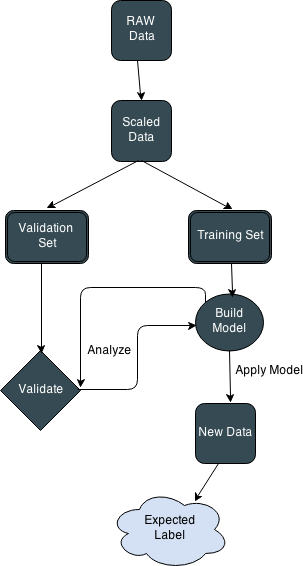
\includegraphics[width=38mm,scale=0.3]{./img/SL.png}
    \caption{\footnotesize{An overview of Supervised learning model that divides scaled data into two sets in order to build a model and predict unseen data }}
    \label{fig:SL}
\end{figure}

In unsupervised learning, no associated label, which is the desired output for a set of inputs, is given to the learning algorithm. The class belonging to each instance in the dataset is unknown and there is no reward when the classifier picks the right class. This technique is therefore more often used when trying to discover hidden classes in new datasets \cite{maglogiannis2007emerging}.








\subsection{Support Vector Machines}
%
Support Vector Machines(SVMs) is a classifier which outputs an optimal hyperplane or set of hyperplanes in high-dimensional space and classifies new examples(unseen data). In other words, SVMs are supervised learning models that employs learning algorithms to recognize patterns and analyze data, used for classification of unknown data\cite{wiki:SVM}.\\
In figure \ref{fig:SVM} main idea behind SVMs is shown. Consider example dataset described by variables $x_1$ and $x_2$. The operation of SVM algorithm is based on finding the optimal hyperplane between training examples. An optimal hyperplane is the one that gives largest minimum distance to the training examples and It maximizes the margin of training data\cite{opencv_library}.

\begin{figure}[H]
    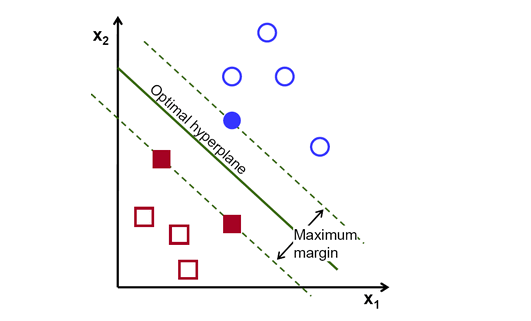
\includegraphics[width=80mm]{./img/SVM.png}
     \caption{Optimal Separating Hyperplane}
    \label{fig:SVM}
\end{figure}

In recent years, SVMs are widely used in bio-informatics \cite{furey2000support,osuna1997training,guyon2002gene} and other discipline due to its ability to accurately deal with high dimensional data\cite{joachims1998text}. They are popular for couple of theoretical reasons: SVMs are robust to very large number of variables and can learn both simple and complex classification models\cite{cristianini2000}.\\

SVMs is a best known member in the general category of kernel methods\cite{shawe2004kernel}. A kernel method has the ability to generate non-linear decision boundaries by using method designed for linear classifiers; This allows the user to apply a classifier to data that has infinite- dimensional vector space representation such as DNA or protein\cite{ben2010user}.    






\subsection{Decision trees}
%A decision tree is a classifier that makes several sequential decisions. The outcome of that sequence determines whether a data point belongs to one class or another. The structure of a decision tree \ref{fig:DT} is defined as a set of nodes ${x_1, ... , x_n}$ with edges ${e_1, .., e_{m}}$ between them. The edges are directed and there are no cycles in the network. The tree has one root $x_1$. With each data point we start at the root. The root node is fed information about a certain feature. The root node then evaluates a rule or function that allows the node to make a decision about what class a data point probably belongs to. Each decision leads to a different node, where another decision is made, increasing the likelihood that the data point belongs to a certain class. This process repeats itself until one of the leaf nodes is reached \cite{safavian1991survey}. From there we can determine what class our initial data point belonged to (either class $A$, $B$ or $C$ in the figure below. 

\begin{figure}[H]
    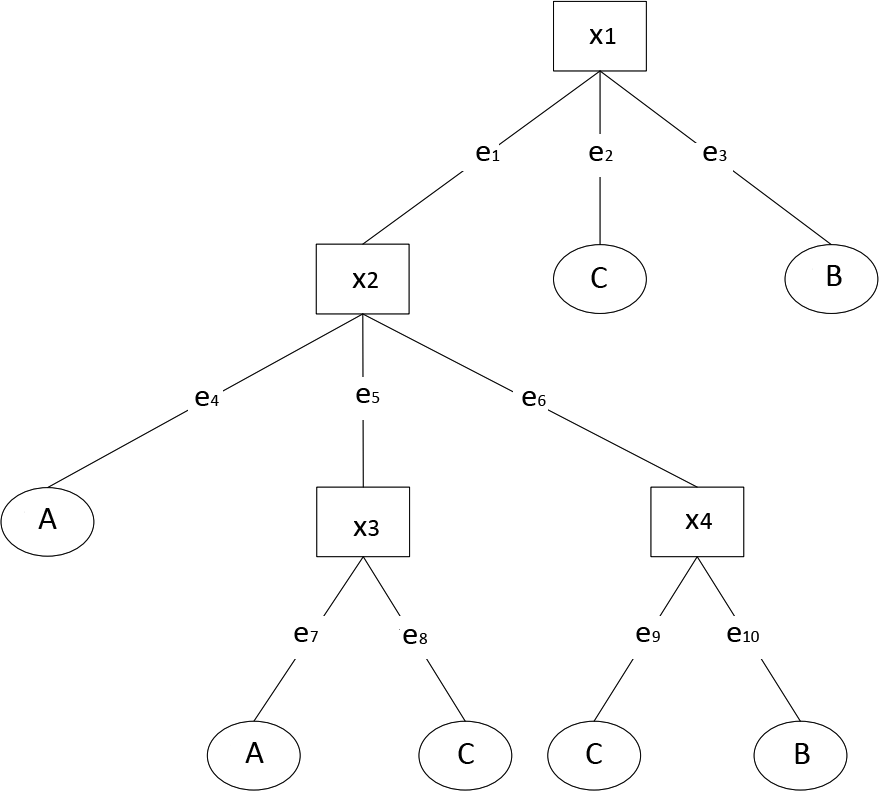
\includegraphics[width=80mm]{./img/decisiontree.png}
    \caption{\footnotesize{Decision Tree example. $x_i$ are nodes where decisions are made. $e_j$ are edges leading down the tree to other nodes. $A,B,C$ are classes that instances are to be classified into.}}
    \label{fig:DT}
\end{figure}

Decision trees are generally built or `grown' with a simple algorithm. Of course random selection of features is an option, but there are many other approaches, like the famous ID3 \cite{quinlan1986induction} and C4.5 algorithm \cite{quinlan1993c4}. ID3 roughly works as follows: We create a node that splits the tree into at least 2 branches. To create a node, we compare every feature and split the one with the highest information gain. In other words, the division will give us a lot of information about the data points and their classes. For example: in classifying trees and plants, height might give more information about which class an instance belongs to than the colour of its leaves would. For each of the subsets that comes forth out of that division, the process is repeated until there is enough certainty that the remaining subset represents the class. This does not take into account that a combination of features might make for an even better split, but it is a relatively efficient algorithm. %Another example of a tree building algorithm is called Fisher's Linear Discriminant Tree \cite{LópezChau20136283}. Fisher's tree is based on maximizing the distance between the means of classes. 

A tree stops to grow when the impurity level is low enough. The impurity level is a metric to indicate what the chances are of misclassification. A simple example for any $node_j$ would be $impurity(node_j) = 1 - max(P(z_i = c_a) $. Here $z_i$ is the $i^{th}$ instance of the subset at our node to be classified into class $c_a$. 

The opposite of growing a tree is called `pruning'. This is done to decrease the complexity of the tree and reduce chance of over fitting. The experts may decide to prune a tree as well if, in hindsight, the training data was faulty in some way. Pruning is done by removing the least significant node(s). 

It is also possible to combine multiple decision trees into a Random Forest \cite{breiman2001random}. This allows for higher accuracy as well as handling higher complexity. Features to split the trees are chosen randomly for each tree. To have enough samples to train the forest, bagging can be performed. Bagging takes random samples from a dataset, with replacement. With this, you have more smaller dataset (with duplicates) that you can train on. With enough trees, the variance of the accuracy decreases. Within forests, every instance to be classified is classified by every tree. The class of an instance is determined by majority vote over all the trees. 

In general, the more nodes a tree has, the more accurate it can be trained. The downside is that the time to classify and train will increase the larger the tree becomes, as well as an increased risk in over fitting. The design of the tree is crucial, as each node splits up the dataset in a certain way. Dividing a datasets in the wrong order can make for significantly slower and less accurate trees. The advantage of the decision tree is it's computational efficiency \cite{safavian1991survey}, its intuitive structure and resistance to noise \cite{LópezChau20136283}.

\subsection{Multi Layer Perceptrons}
\hspace{0.5cm} MultiLayer Perceptrons are a type of supervised learning \cite{michie1994machine}. It is a type of neural network consisting of multiple layers of perceptrons. A perceptron is a system of nodes with input nodes, called the input layer, and an output node called the output layer. Inputs from a vector $x$ are fed to the input layer with weights $w$. Within the perceptron, each input value is compared with a certain function and increased by a certain weight. The output is determined based on the threshold
\begin{figure}[h!]
  \caption{Rosenblatt's perceptron}
  \centering
    
\includegraphics[width=55mm]{./img/perceptron.png}
    \label{fig:perceptron}
\end{figure}

%------------------------------------------------

\section{Comparison of classifiers}
\subsection{SVM Vs DT} % (fold)
It is impossible to fully compare Support Vector Machines and Decision Trees. Both have advantages and disadvantages, each serving it's own purpose. One such difference is that DTs are faster when handling new datasets, compared to SVM. This is because of the complexity of SVMs' arithmetic computations, where DTs only need to follow a logical path in a tree. A more interesting difference is that SVM has higher accuracy in general as was observed in numerous studies\cite{arun2010hybrid}.
 
A study more closely related to SAR used hydro acoustics to classify different species of fish. Sonar is used to create hydro acoustic images, which results in similar images as SAR \cite{griffiths2003synthetic}. Fourteen features were used. Both SVM and DT were considered good classifiers. SVM required more preprocessing time, but had slightly higher results. DT was easier to implement and easier to read. However, DT showed greater variance \cite{Robotham2011170}.

SVM and DTs were also compared in a study using LandSat images. They used SVM, DT and Maximum Likelihood Classifier (MLC) to determine different types of land coverage (e.g. forest, water, wetlands, open grasland) in Uganda. Though the spatial dimension of LandSat (which produces optical/visual images) is lower than the average SAR satellite, there are a lot of similarities. Out of eight classes, both SVM and DT were able to distinguish seven classes. DT had a slightly higher accuracy rate and higher kappa statistic \cite{Otukei2010S27}.




\subsection{SVM Vs MLP} % (fold)
SVM and MLP are two known classifiers that has lots of potential to truthfully predict classification solutions. According to Wolpert and Macready, in their paper\cite{wolpert1995no}, they have indicated that `any two optimization algorithms are equivalent when their performance is averaged across all possible problems'. This makes it difficult to choose a supreme classifier.  Researchers\cite{Moavenian20103088,Zanaty2012177} has practiced some experiments to know which classifier might predict more accurate than other; the outcome of this experiments indicated that SVM outperforms MLP in one case while In another type of dataset SVM falls below MLP. If a comparison is done theoretically then SVM and MLP has their own distinguishing advantages. SVM classifiers has a strong founding theory and need less memory to store the predictive model; Even when training sample has some bias, If the right parameters are chosen for SVM, then it can be robust\cite{auria2008support} but advantages of MLP are not as few as SVM. MLPs are popular in machine learning solutions such as speech recognition, image recognition because of their ability to solve problems stochastically, meaning that it allows user to get approximate solution for very complex problems like fitness approximation\cite{jin2005neural}. Here we will look closely at SVM and MLP performance using real world dataset in various disciplines(ECG arrhythmias,text recognition, remote sensing, wind speed prediction) to examine performance of them. It is obvious here that free lunch theorem\cite{wolpert1995no} is valid, sine there is no superior classifier to other in all cases!\\
In the field of ECG(Electrocardiography), comparison between MLP and SVM is done using same dataset. MLP accuracy in classifying the ECG(Electrocardiography) signals, is more accurate than other ANN. MLP with back propagation(BP) training algorithm suffer from slow convergence to local minima, on the other hand SVM classifier with (K-A) training do not trap in local minima points therefore they are faster than ANN\cite{Moavenian20103088}.\\
 In high dimensional data, SVM accomplishes better accuracy compare to MLP, this is when new kernel function proposed for SVM. The reason behind is that MLP needs more hidden units for tested data set and become more complex when the dimension of data set increases whereas SVM complexity does not depend on dimension of data set. SVM are efficient on optimal separation of unseen data points\cite{Zanaty2012177}.\\
SVM works better than MLP for the off-line signature recognition(within finite database). The comparison is done between the identification rate(increment of 20\% for SVM) and for training time needed. The superiority of SVM is because of its generalization ability in high dimensional space\cite{FriasMartinez2006693}.\\
SVM outperforms to MLP, in Wind speed prediction. The comparison is done using a wind speed dataset that cover a 12 years between 1970-1982. Dataset is divided into three parts: training, test and validation sets. The output result shown the SVM outperform MLP on all orders resulting in the lower MSE(MLP is 0.0090 while it is 0.0078)\cite{Mohandes2004939}.\\
In oil spill detection, the datasets are imbalanced, in which most instances(that are not oil spill spot) belong to a larger class and very few instances for smaller class(oil spill spot). Lack of instances in minority class will cause SVM suffer from biased decision boundary and prediction performance, however combining SVM with an over-sampling and under-sampling technique will make SVM outperform to other classifiers\cite{liu2006boosting}.

	
      




	
\subsection{DT Vs MLP}
\begin{itemize}
	
	\item  In \cite{Mera2014} a Decision Support System to detect oil spills has been created. For classification both a neural network and a decision tree are used. Since both classifiers are designed and tested using the same data, a comparison on accuracy can be made. The neural network appears to outperform the decision tree slightly.\cite{Moavenian20103088}
	
	\item  Another study by \cite{Xu2014} also compared different classifers for oil spill detection. Here they experienced an opposite result. Out of seven classifiers, the ANN was found to perform the worst by 14.8 percentage points. The results indicated that the additional flexibility provided by SVM and ANN does not necessarily improve the predicitive performance compared to less flexible methods. Both tend to overfit the dataset on small-sized training samples and could not generalize well.
    

\end{itemize}



	

\section{Discussion}
\section{Final words or conclusion}

%\input{./sections/12.conclusion.tex}
\end{multicols}

\newpage
%----------------------------------------------------------------------------------------
%	REFERENCE LIST
%----------------------------------------------------------------------------------------

\bibliographystyle{plain}
\bibliography{refrences}
%----------------------------------------------------------------------------------------




\end{document}